\section{Testing eBPF programs}\label{sec:testing}
To verify the correctness of a P4-XDP program, the compiler integrates a full 
end-to-end testing framework. The framework consists of an userspace eBPF 
runtime as well as a kernel testing pipeline, which verifies eBPF/XDP programs 
in a virtual, isolated environment.

\subsection{Why Test in User-Space?}
Testing in user space isolates the specification of the eBPF program from the 
implementation. It is primarily intended to test the correctness of the 
compiler and the generated C code without interference of the kernel verifier 
and tooling. The user space testing framework does not depend on the LLVM 
compiler or specific kernel version. It also does not require usage of tools 
such as tc or ip. The goal is to ensure that a P4 program is functionally 
equivalent to its corresponding XDP C-code.
Testing in user space also guarantees debugging simplicity for the average 
user. Tools such as GDB, valgrind, wireshark, or simple debugging statements 
are readily available.
 
\subsection{The Simple Test Framework}
\begin{figure}
	\centering
	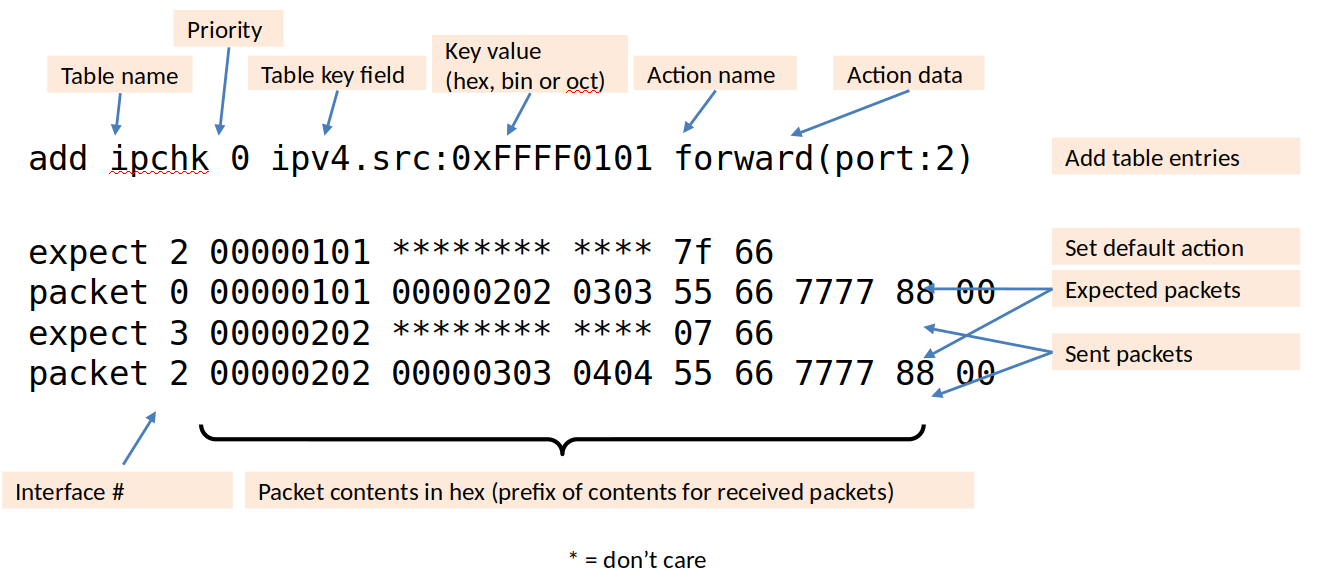
\includegraphics[width=0.7\linewidth]{stf}
	\caption{}
	\label{fig:stf}
\end{figure}
The simple test framework (STF) is a data plane verification language, which is 
used by the p4c-ebpf compiler. While its original purpose is to assess 
switching and 
forwarding behavior, it can also test the functionality of eBPF programs in 
isolation.
In general, an STF file describes the input as well the expected output 
packets per switch, or in this case virtual bridge, port.

\begin{table}[h]
	\begin{center}
		\begin{tabular}{|l|l|} \hline
			\textbf{Command} & \textbf{Description} \\ \hline \hline
			\textbf{packet} port data & Insert a frame of bytes 
			\textit{data} into port \textit{port}.    \\ \hline
			\textbf{expect} port data & Expect a frame of bytes 
			\textit{data} on port \textit{port}.  \\ \hline
			\textbf{add} tbl priority match action & Insert a 
			match-action entry with key \textit{match} and action 
			\textit{action} into table \textit{tbl}. \\ \hline
			\textbf{setdefault} tbl action & Set the default action for table 
			\textit{tbl}. \\ 
			\hline
			\textbf{check\_counter} tbl\_name key == n & Check if the value on 
			the entry \textit{key} in counter table \textit{tbl} matches 
			\textit{n}.  \\ 
			\hline
			\textbf{wait} & Pause any operation for a second. \\ \hline
		\end{tabular}
		\caption{The STF command palette.}\label{table:stf}
	\end{center}
\end{table}


Compiler comes with a Python parser for STF

\subsection{The Test Runtime}
Describe the userspace runtime.
User-space wrappers around eBPF tables and APIs
\begin{figure}
	\centering
	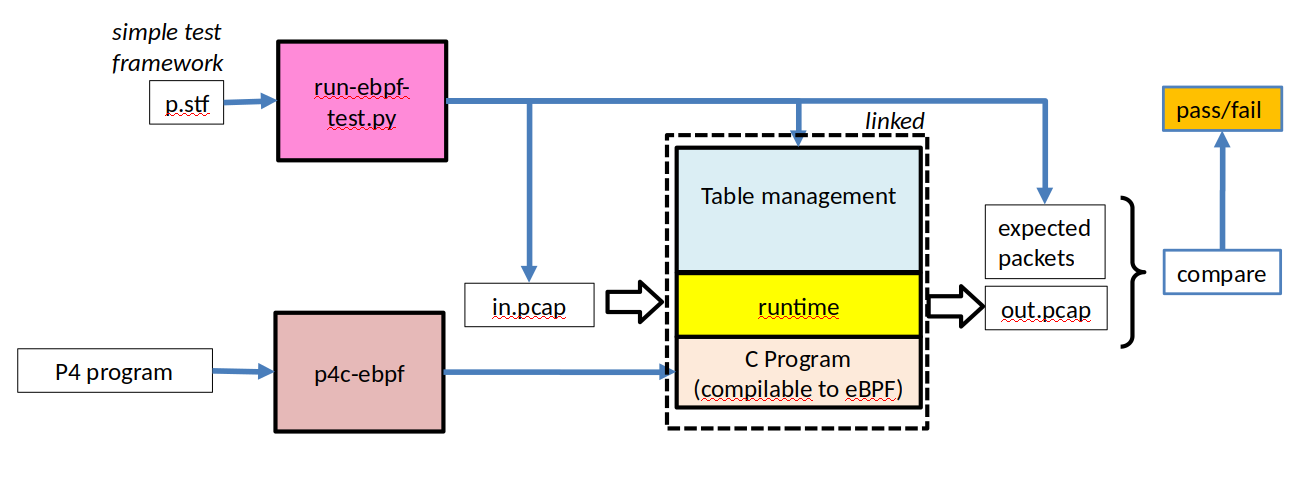
\includegraphics[width=0.7\linewidth]{user_test}
	\caption{}
	\label{fig:user_test}
\end{figure}

\subsection{Testing P4 Programs End-to-End}
Talk about how to use the test framework to verify your eBPF code or p4 file 
end-to-end. Highlight, how the framework can be used to test eBPF and XDP 
programs in general, independent from the P4 pipeline.
\begin{figure}
	\centering
	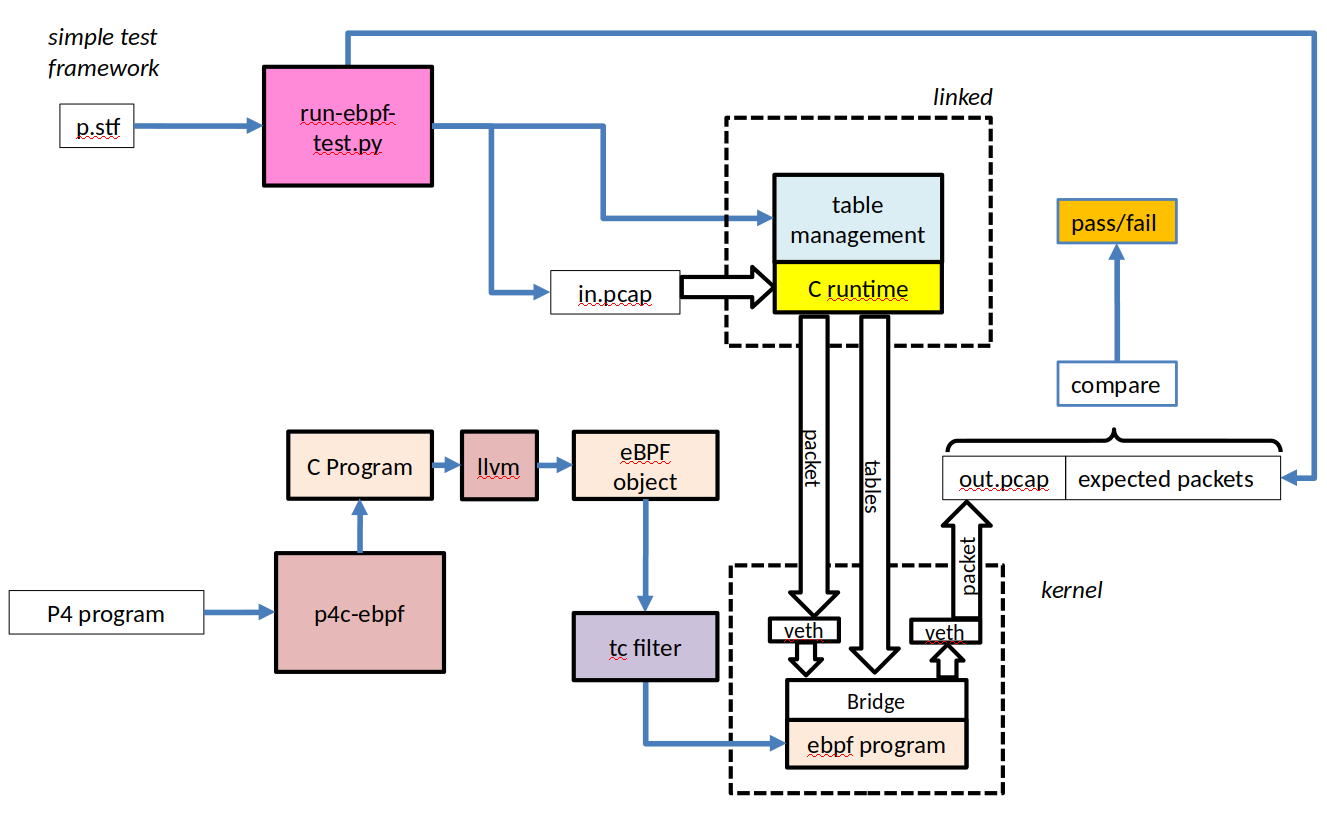
\includegraphics[width=0.7\linewidth]{kernel_test}
	\caption{}
	\label{fig:kernel_test}
\end{figure}